\documentclass[letterpaper,11pt,oneside,reqno]{amsart}
\usepackage[numbers,sort&compress]{natbib}
\usepackage{rotating}
\usepackage{graphicx}
\usepackage[utf8]{inputenc}
\usepackage[english]{babel}
\usepackage{xcolor}
\usepackage{bm}
\usepackage{caption}
\usepackage{afterpage}
\usepackage{enumitem}
%\usepackage[dvipdfmx]{graphicx} 
\usepackage{bmpsize}
\usepackage{hyperref}

%%%%%%%%%%%%%%%%%%%%%%%%%%%%%%%%%%%%%%%%%%%%%%%%%%%%%%%%%%%%
%main packages
\usepackage{amsmath,amssymb,amsthm,amsfonts, dsfont}
\usepackage{relsize}
\usepackage{graphicx,color,subcaption}
\usepackage{upgreek}
\usepackage[mathscr]{euscript}

%equations
\allowdisplaybreaks
\numberwithin{equation}{section}

%tikz
\usepackage{tikz}
\usetikzlibrary{arrows,positioning,decorations.markings}

%conveniences
\usepackage{float}
\usepackage{multicol}
\usepackage{array}
\usepackage{adjustbox}
\usepackage{cleveref}
%paper geometry
\usepackage[DIV=12]{typearea}
\synctex=1
\newtheorem{proposition}{Proposition}[section]
\newtheorem{lemma}[proposition]{Lemma}
\newtheorem{corollary}[proposition]{Corollary}
\newtheorem{theorem}[proposition]{Theorem}
\newtheorem{maintheorem}{Theorem}
\newtheorem{mainprop}[maintheorem]{Proposition}
%%%%%%%%%%%%%%%%%%%%%%%%%%%%%%%%%%%%%%%%%%%%%%%%%%%%%%%%%%%%
\theoremstyle{definition}
\newtheorem{definition}[proposition]{Definition}
\newtheorem{remark}[proposition]{Remark}
%%%%%%%%%%%%%%%%%%%%%%%%%%%%%%%%%%%%%%%%%%%%%%%%%%%%%%%%%%%%
\newtheoremstyle{qqq}
{}   % ABOVESPACE
{}   % BELOWSPACE
{\slshape}  % BODYFONT
{0pt}       % INDENT (empty value is the same as 0pt)
{\bfseries} % HEADFONT
{.}         % HEADPUNCT
{5pt plus 1pt minus 1pt} % HEADSPACE
{}          % CUSTOM-HEAD-SPEC
\theoremstyle{qqq}
\newtheorem{question}[proposition]{Open problem}
%%%%%%%%%%%%%%%%%%%%%%%%%%%%%%%%%%%%%%%%%%%%%%%%%%%%%%%%%%%%

\makeatletter
\newcommand*{\da@rightarrow}{\mathchar"0\hexnumber@\symAMSa 4B }
\newcommand*{\da@leftarrow}{\mathchar"0\hexnumber@\symAMSa 4C }
\newcommand*{\xdashrightarrow}[2][]{%
	\mathrel{%
		\mathpalette{\da@xarrow{#1}{#2}{}\da@rightarrow{\,}{}}{}%
	}%
}
\newcommand{\xdashleftarrow}[2][]{%
	\mathrel{%
		\mathpalette{\da@xarrow{#1}{#2}\da@leftarrow{}{}{\,}}{}%
	}%
}
\newcommand*{\da@xarrow}[7]{%
	% #1: below
	% #2: above
	% #3: arrow left
	% #4: arrow right
	% #5: space left 
	% #6: space right
	% #7: math style 
	\sbox0{$\ifx#7\scriptstyle\scriptscriptstyle\else\scriptstyle\fi#5#1#6\m@th$}%
	\sbox2{$\ifx#7\scriptstyle\scriptscriptstyle\else\scriptstyle\fi#5#2#6\m@th$}%
	\sbox4{$#7\dabar@\m@th$}%
	\dimen@=\wd0 %
	\ifdim\wd2 >\dimen@
	\dimen@=\wd2 %   
	\fi
	\count@=2 %
	\def\da@bars{\dabar@\dabar@}%
	\@whiledim\count@\wd4<\dimen@\do{%
		\advance\count@\@ne
		\expandafter\def\expandafter\da@bars\expandafter{%
			\da@bars
			\dabar@ 
		}%
	}%  
	\mathrel{#3}%
	\mathrel{%   
		\mathop{\da@bars}\limits
		\ifx\\#1\\%
		\else
		_{\copy0}%
		\fi
		\ifx\\#2\\%
		\else
		^{\copy2}%
		\fi
	}%   
	\mathrel{#4}%
}
\makeatother
%\makeatletter
%\def\@fnsymbol#1{\ensuremath{\ifcase#1\or *\or \dagger\or **\or
%   \ddagger\or \mathsection\or \mathparagraph\or \|\or \dagger\dagger
%   \or \ddagger\ddagger \or\mathsection\mathsection
%   \or \mathparagraph\mathparagraph \or *{*}*\or
%   \dagger{\dagger}\dagger \or\ddagger{\ddagger}\ddagger\or
%   \mathsection{\mathsection}\mathsection
%   \or \mathparagraph{\mathparagraph}\mathparagraph \else\@ctrerr\fi}}
%\makeatother

% Document starts
\begin{document}

% Title portion
\title{Shock-wave Thickness Influence to the Light Diffraction on a Plane Shock Wave}

\author{Maksim Timokhin}
\address{M. Timokhin, Lomonosov Moscow State University, 119991, Moscow, Russia and Moscow Aviation Institute, 125993, Moscow, Russia}
\email{timokhin@physics.msu.ru}
\author{Mikhail Tikhonov}
\address{M. TIkhonov, Lomonosov Moscow State University, 119991, Moscow, Russia}
\author{Irina Mursenkova}
\address{I. Mursenkova, Lomonosov Moscow State University, 119991, Moscow, Russia}
\author{Irina Znamenskaya}
\address{I. Znamenskaya, Lomonosov Moscow State University, 119991, Moscow, Russia}




\begin{abstract}
	to be written
\end{abstract}
\date{}

\maketitle

\setcounter{tocdepth}{3}

% Head 1
\section{INTRODUCTION}

Optical methods of gas-dynamic flow visualization are based on a change in the optical path of light through inhomogeneities in the density of a transparent medium. Such optical methods include shadowgraph, schlieren, and interferometric methods \cite{}. Shadowgraph methods are most often used to visualize shock waves and to experimentally analyze shock-wave configurations \cite{}. At the same time, usually the aim of applying this approach is to fix the positions of the shock waves. 

In classical gas dynamics of inviscid gas shock waves are treated as discontinuities \citep{Sedov,LANDAU1987}. This fact implies that the average mean free path tends to zero in comparison with the flow scale. 

A rather simple method was proposed for numerically calculating the result of light diffraction by a plane shock of zero thickness in \cite{Pfeifer}. A jump in density leads to a jump in the refractive index of the medium and to a jump in the phase of the wave. A similar approach was used, for example, in \cite{Panda_1995} to calculate the light intensity after passing through a shock wave in front of a blunt body. The obtained numerical results of light intensity distribution on the screen are in excellent agreement with the presented experimental shadowgraph data \cite{Pfeifer,Panda_1995}.

It is well-known fact that for sufficiently dilute gases the shock-wave thickness constitutes several mean free paths (see e.g. \cite{Kogan, Cercignani_book}). Here we would like to investigate the shock thickness influence on the light diffraction results. The shock-wave structure problem has been studied analytically with different mathematical approaches \cite{Becker_1922, Mott-Smith_1951, Salwen_1964, Holway_1964, Yen_1966}. The structure of a plane shock wave has been investigated experimentally with optical and electron methods fluorescence methods \cite{Hornig_1950, Hansen_Hornig_1960, Robben, Alsmeyer_1976, Pham-Van-Diep624}. A lot of investigations were provided with kinetic approach. The numerical results of this approach, as well as the experimental data, became the reference for this flow. This way includes the numerical solution of Boltzmann kinetic equation  \citep{Ohwada_shock, Dodulad_Tcheremissine_2013, ShockWaves_2015}, model kinetic equations \citep{Shakhov, Rykov2008} and Direct Simulation Monte Carlo (DSMC) method \citep{Belotserkovskii, Pham-Van-Diep624, Erofeev_Friedlander_overshoot_2002, overshoot_2015}.

\section{PROBLEM FORMULATION AND MATHEMATICAL MODEL}

The values of the amplitude and phase are first determined at equidistant points immediately after the passage of the diffraction object. These points, by virtue of the Huygens-Fresnel principle, will be sources of secondary waves, the result of which is summed up at each observation point in accordance with their optical paths. Due to the one-dimensionality of the shock wave, cylindrical waves are used instead of spherical ones.

\begin{figure}
\begin{tabular}{cc}
    {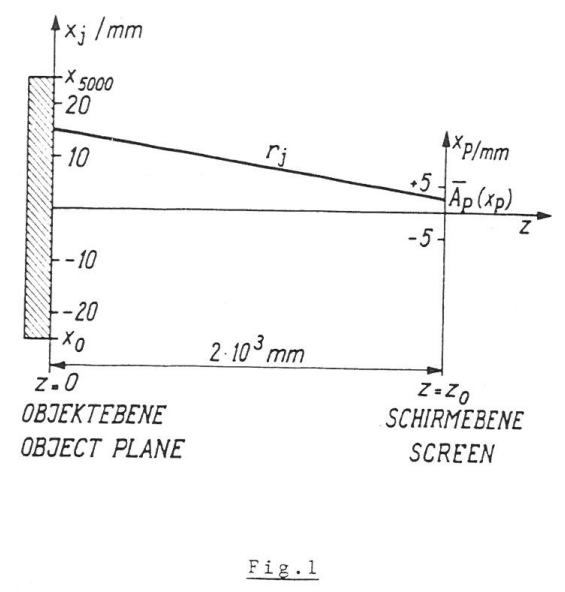
\includegraphics[width=160pt]{fig1.png}}
    &{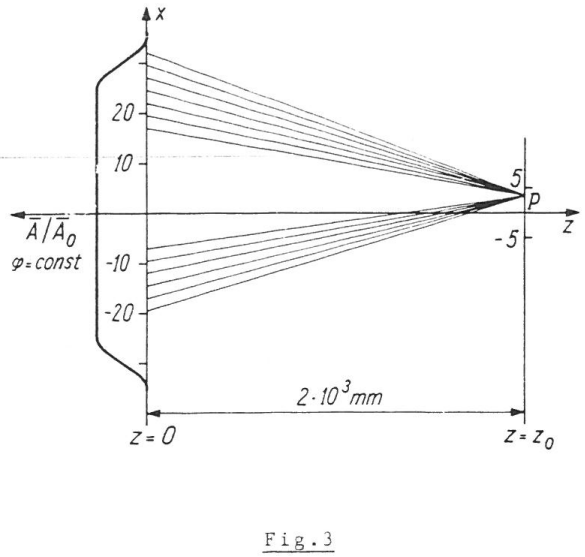
\includegraphics[width=160pt]{fig3.png}}\\ a&b
\end{tabular}
\label{Formulation}
\end{figure}

In the plane of the object $z=0$, according to the Fig. \ref{Formulation} a, the density of the source points is more than 100 points per millimeter. Thus, with the assumed incident width, 50 mm plane wavefront, and distance $z_0 = 2$ m, more than two reference points are taken into account even in the outermost Fresnel zone. The complex amplitude $\overline{A}_p$ at the point $P{(x_p, z_0)}$ on the screen at the distance of $z_0$ from the plane of the object is calculated by the formula:
\begin{equation}
\overline{A}_p = \sum_{j=1}^{n} A_j \left(\frac{z_0}{r_j} \right)^{1/2} \exp \left(i \frac{2\pi}{\lambda} \left(r_j - z_0\right) + \Phi_j\right)
\end{equation}

where $n$ is the number of source points, $A_j$ is the magnitude of the amplitude at the $j$-th point, $\Phi_j$ is the initial phase at the $j$-th point and $\lambda$ is the light wavelength. $r_j$ is  defined as: $r_j = \left(z_0^2 + \left(x_j - x_P\right)^2\right)^{1/2}$. $x_j$ is the current coordinate at the plane near the diffraction object.


As a validation of the numerical implementation the method, initially the test and experimental results from \cite{Pfeifer} were exactly reproduced.



\subsection{EXPERIMENTAL SETUP}


\section{RESULTS}

\subsection{Experimental case}

In Fig. \ref{Experiment_Ma2p1} a presents a shadow photograph obtained using the experimental setup described above. The shock wave moves from left to right. The pressure and temperature in front of the shock wave on the right are $p_0=25$ Torr and $T_0=293$ K, respectively. The Mach number of the shock wave is $Ma=2.1$. Fig. \ref{Experiment_Ma2p1} b shows the distribution of light intensity in the experiment obtained from \ref{Experiment_Ma2p1} a.

\begin{figure}
\begin{tabular}{cc}
    {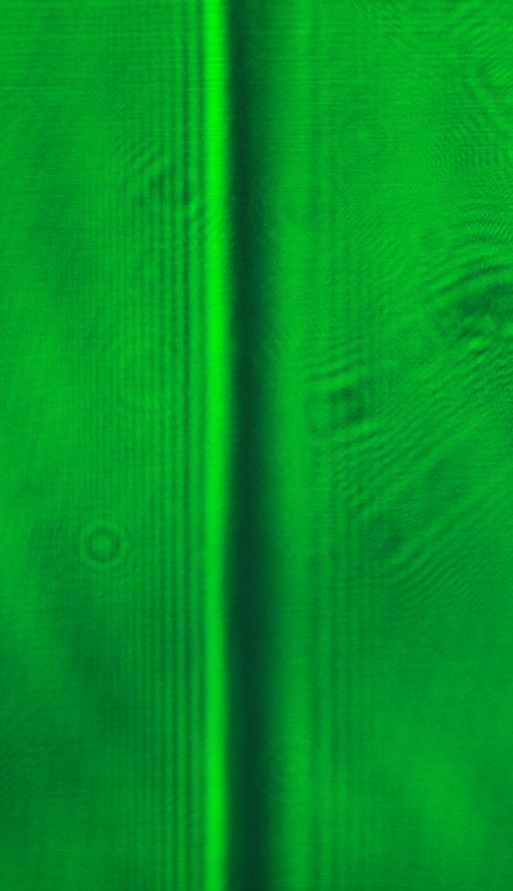
\includegraphics[width=185pt, height=100pt]{Experiment_Ma2p1_foto.jpg}}
    &{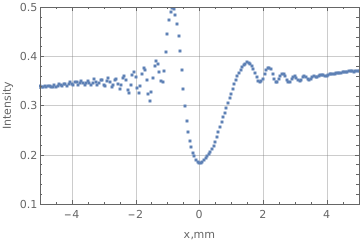
\includegraphics[width=185pt,height=100pt]{2b.png}}\\ a&b
\end{tabular}
\caption{The shadowgraph image for $Ma=2.1$, $p_0=25$ Torr and $T_0=293$ K (a) and its intensity distribution {b}.}
\label{Experiment_Ma2p1}
\end{figure}



\subsection{The dependence on shock thickness}


\section{CONCLUSION}

% Acknowledgement
\section{ACKNOWLEDGMENTS}
The work carried out at Moscow State University was supported by the Russian Science Foundation (Grant No. ).

% References

%merlin.mbs aipnum4-1.bst 2010-07-25 4.21a (PWD, AO, DPC) hacked
%Control: key (0)
%Control: author (8) initials jnrlst
%Control: editor formatted (1) identically to author
%Control: production of article title (-1) disabled
%Control: page (0) single
%Control: year  (1) truncated
%Control: production of eprint (0) enabled
\begin{thebibliography}{41}%
	\makeatletter
	\providecommand \@ifxundefined [1]{%
		\@ifx{#1\undefined}
	}%
	\providecommand \@ifnum [1]{%
		\ifnum #1\expandafter \@firstoftwo
		\else \expandafter \@secondoftwo
		\fi
	}%
	\providecommand \@ifx [1]{%
		\ifx #1\expandafter \@firstoftwo
		\else \expandafter \@secondoftwo
		\fi
	}%
	\providecommand \natexlab [1]{#1}%
	\providecommand \enquote  [1]{``#1''}%
	\providecommand \bibnamefont  [1]{#1}%
	\providecommand \bibfnamefont [1]{#1}%
	\providecommand \citenamefont [1]{#1}%
	\providecommand \href@noop [0]{\@secondoftwo}%
	\providecommand \href [0]{\begingroup \@sanitize@url \@href}%
	\providecommand \@href[1]{\@@startlink{#1}\@@href}%
	\providecommand \@@href[1]{\endgroup#1\@@endlink}%
	\providecommand \@sanitize@url [0]{\catcode `\$12\catcode `\&12\catcode
		`\#12\catcode `\^12\catcode `\_12\catcode `\%12\relax}%
	\providecommand \@@startlink[1]{}%
	\providecommand \@@endlink[0]{}%
	\providecommand \url  [0]{\begingroup\@sanitize@url \@url }%
	\providecommand \@url [1]{\endgroup\@href {#1}{\urlprefix }}%
	\providecommand \urlprefix  [0]{URL }%
	\providecommand \Eprint [0]{\href }%
	\providecommand \doibase [0]{http://dx.doi.org/}%
	\providecommand \selectlanguage [0]{\@gobble}%
	\providecommand \bibinfo  [0]{\@secondoftwo}%
	\providecommand \bibfield  [0]{\@secondoftwo}%
	\providecommand \translation [1]{[#1]}%
	\providecommand \BibitemOpen [0]{}%
	\providecommand \bibitemStop [0]{}%
	\providecommand \bibitemNoStop [0]{.\EOS\space}%
	\providecommand \EOS [0]{\spacefactor3000\relax}%
	\providecommand \BibitemShut  [1]{\csname bibitem#1\endcsname}%
	\let\auto@bib@innerbib\@empty
	%</preamble>
	\bibitem [{\citenamefont {Panda}\ and\ \citenamefont
		{Adamovsky}(1995)}]{Panda_1995}%
	\BibitemOpen
	\bibfield  {author} {\bibinfo {author} {\bibfnamefont {J.}~\bibnamefont
			{Panda}}\ and\ \bibinfo {author} {\bibfnamefont {G.}~\bibnamefont
			{Adamovsky}},\ }\href {\doibase 10.1063/1.868475} {\bibfield  {journal}
		{\bibinfo  {journal} {Physics of Fluids}\ }\textbf {\bibinfo {volume} {7}},\
		\unskip\ \bibinfo {pages} {2271--2279} (\bibinfo {year} {1995})},\ \Eprint
	{http://arxiv.org/abs/https://doi.org/10.1063/1.868475}
	{https://doi.org/10.1063/1.868475} \BibitemShut {NoStop}%
	\bibitem [{\citenamefont {Schmidt}(1969)}]{Schmidt_1969}%
	\BibitemOpen
	\bibfield  {author} {\bibinfo {author} {\bibfnamefont {B.}~\bibnamefont
			{Schmidt}},\ }\href@noop {} {\bibfield  {journal} {\bibinfo  {journal} {J.
				Fluid Mech.}\ }\textbf {\bibinfo {volume} {39}},\ \unskip\ \bibinfo {pages}
		{361--–373} (\bibinfo {year} {1969})}\BibitemShut {NoStop}%
	\bibitem [{\citenamefont {Alsmeyer}(1976)}]{Alsmeyer_1976}%
	\BibitemOpen
	\bibfield  {author} {\bibinfo {author} {\bibfnamefont {H.}~\bibnamefont
			{Alsmeyer}},\ }\href@noop {} {\bibfield  {journal} {\bibinfo  {journal} {J.
				Fluid Mech.}\ }\textbf {\bibinfo {volume} {74}},\ \unskip\ \bibinfo {pages}
		{497--–513} (\bibinfo {year} {1976})}\BibitemShut {NoStop}%
	\bibitem [{\citenamefont {Pham-Van-Diep}, \citenamefont {Erwin},\ and\
		\citenamefont {Muntz}(1989)}]{Pham-Van-Diep624}%
	\BibitemOpen
	\bibfield  {author} {\bibinfo {author} {\bibfnamefont {G.}~\bibnamefont
			{Pham-Van-Diep}}, \bibinfo {author} {\bibfnamefont {D.}~\bibnamefont
			{Erwin}}, \ and\ \bibinfo {author} {\bibfnamefont {E.~P.}\ \bibnamefont
			{Muntz}},\ }\href {\doibase 10.1126/science.245.4918.624} {\bibfield
		{journal} {\bibinfo  {journal} {Science}\ }\textbf {\bibinfo {volume}
			{245}},\ \unskip\ \bibinfo {pages} {624--626} (\bibinfo {year}
		{1989})}\BibitemShut {NoStop}%
	\bibitem [{\citenamefont {Becker}(1922)}]{Becker_1922}%
	\BibitemOpen
	\bibfield  {author} {\bibinfo {author} {\bibfnamefont {R.}~\bibnamefont
			{Becker}},\ }\href@noop {} {\bibfield  {journal} {\bibinfo  {journal} {Z.
				Phys.}\ }\textbf {\bibinfo {volume} {8}},\ \unskip\ \bibinfo {pages}
		{321--362} (\bibinfo {year} {1922})}\BibitemShut {NoStop}%
	\bibitem [{\citenamefont {Mott-Smith}(1951)}]{Mott-Smith_1951}%
	\BibitemOpen
	\bibfield  {author} {\bibinfo {author} {\bibfnamefont {H.~M.}\ \bibnamefont
			{Mott-Smith}},\ }\href@noop {} {\bibfield  {journal} {\bibinfo  {journal}
			{Phys. Rev.}\ }\textbf {\bibinfo {volume} {82}},\ \unskip\ \bibinfo {pages}
		{885--–892} (\bibinfo {year} {1951})}\BibitemShut {NoStop}%
	\bibitem [{\citenamefont {Salwen}, \citenamefont {Grosch},\ and\ \citenamefont
		{Ziering}(1964)}]{Salwen_1964}%
	\BibitemOpen
	\bibfield  {author} {\bibinfo {author} {\bibfnamefont {H.}~\bibnamefont
			{Salwen}}, \bibinfo {author} {\bibfnamefont {C.~E.}\ \bibnamefont {Grosch}},
		\ and\ \bibinfo {author} {\bibfnamefont {S.}~\bibnamefont {Ziering}},\ }\href
	{\doibase 10.1063/1.1711131} {\bibfield  {journal} {\bibinfo  {journal} {The
				Physics of Fluids}\ }\textbf {\bibinfo {volume} {7}},\ \unskip\ \bibinfo
		{pages} {180--189} (\bibinfo {year} {1964})},\ \Eprint
	{http://arxiv.org/abs/https://aip.scitation.org/doi/pdf/10.1063/1.1711131}
	{https://aip.scitation.org/doi/pdf/10.1063/1.1711131} \BibitemShut {NoStop}%
	\bibitem [{\citenamefont {Kogan}(1969)}]{Kogan}%
	\BibitemOpen
	\bibfield  {author} {\bibinfo {author} {\bibfnamefont {M.}~\bibnamefont
			{Kogan}},\ }\href@noop {} {\emph {\bibinfo {title} {Rarefied gas dynamics}}}\
	(\bibinfo  {publisher} {Plenum},\ \bibinfo {address} {New York},\ \bibinfo
	{year} {1969})\BibitemShut {NoStop}%
	\bibitem [{\citenamefont {Dodulad}\ and\ \citenamefont
		{Tcheremissine}(2013)}]{Dodulad_Tcheremissine_2013}%
	\BibitemOpen
	\bibfield  {author} {\bibinfo {author} {\bibfnamefont {O.~I.}\ \bibnamefont
			{Dodulad}}\ and\ \bibinfo {author} {\bibfnamefont {F.~G.}\ \bibnamefont
			{Tcheremissine}},\ }\href@noop {} {\bibfield  {journal} {\bibinfo  {journal}
			{Comput. Math. Math. Phys.}\ }\textbf {\bibinfo {volume} {53}},\ \unskip\
		\bibinfo {pages} {827--–844} (\bibinfo {year} {2013})}\BibitemShut
	{NoStop}%
	\bibitem [{\citenamefont {Rykov}, \citenamefont {Titarev},\ and\ \citenamefont
		{Shakhov}(2008)}]{Rykov2008}%
	\BibitemOpen
	\bibfield  {author} {\bibinfo {author} {\bibfnamefont {V.~A.}\ \bibnamefont
			{Rykov}}, \bibinfo {author} {\bibfnamefont {V.~A.}\ \bibnamefont {Titarev}},
		\ and\ \bibinfo {author} {\bibfnamefont {E.~M.}\ \bibnamefont {Shakhov}},\
	}\href {\doibase 10.1134/S0015462808020178} {\bibfield  {journal} {\bibinfo
			{journal} {Fluid Dynamics}\ }\textbf {\bibinfo {volume} {43}},\ \unskip\
		\bibinfo {pages} {316--326}Apr (\bibinfo {year} {2008})}\BibitemShut
	{NoStop}%
	\bibitem [{\citenamefont {Malkov}\ \emph {et~al.}(2015)\citenamefont {Malkov},
		\citenamefont {Bondar}, \citenamefont {Kokhanchik}, \citenamefont
		{Poleshkin},\ and\ \citenamefont {Ivanov}}]{ShockWaves_2015}%
	\BibitemOpen
	\bibfield  {author} {\bibinfo {author} {\bibfnamefont {E.~A.}\ \bibnamefont
			{Malkov}}, \bibinfo {author} {\bibfnamefont {Y.~A.}\ \bibnamefont {Bondar}},
		\bibinfo {author} {\bibfnamefont {A.~A.}\ \bibnamefont {Kokhanchik}},
		\bibinfo {author} {\bibfnamefont {S.}~\bibnamefont {Poleshkin}}, \ and\
		\bibinfo {author} {\bibfnamefont {M.}~\bibnamefont {Ivanov}},\ }\href@noop {}
	{\bibfield  {journal} {\bibinfo  {journal} {Shock Waves}\ }\textbf {\bibinfo
			{volume} {25}},\ \unskip\ \bibinfo {pages} {387--397} (\bibinfo {year}
		{2015})}\BibitemShut {NoStop}%
	\bibitem [{\citenamefont {Torrilhon}\ and\ \citenamefont
		{Struchtrup}(2004)}]{Struchtrup_Torrilhon_2004}%
	\BibitemOpen
	\bibfield  {author} {\bibinfo {author} {\bibfnamefont {M.}~\bibnamefont
			{Torrilhon}}\ and\ \bibinfo {author} {\bibfnamefont {H.}~\bibnamefont
			{Struchtrup}},\ }\href {\doibase 10.1017/S0022112004009917} {\bibfield
		{journal} {\bibinfo  {journal} {Journal of Fluid Mechanics}\ }\textbf
		{\bibinfo {volume} {513}},\ p.\ \bibinfo {pages} {171–198} (\bibinfo {year}
		{2004})},\ \Eprint
	{http://arxiv.org/abs/https://doi.org/10.1017/S0022112004009917}
	{https://doi.org/10.1017/S0022112004009917} \BibitemShut {NoStop}%
	\bibitem [{\citenamefont {Timokhin}\ \emph {et~al.}(2015)\citenamefont
		{Timokhin}, \citenamefont {Bondar}, \citenamefont {Kokhanchik}, \citenamefont
		{Ivanov}, \citenamefont {Ivanov},\ and\ \citenamefont
		{Kryukov}}]{overshoot_2015}%
	\BibitemOpen
	\bibfield  {author} {\bibinfo {author} {\bibfnamefont {M.~Y.}\ \bibnamefont
			{Timokhin}}, \bibinfo {author} {\bibfnamefont {Y.~A.}\ \bibnamefont
			{Bondar}}, \bibinfo {author} {\bibfnamefont {A.~A.}\ \bibnamefont
			{Kokhanchik}}, \bibinfo {author} {\bibfnamefont {M.~S.}\ \bibnamefont
			{Ivanov}}, \bibinfo {author} {\bibfnamefont {I.~E.}\ \bibnamefont {Ivanov}},
		\ and\ \bibinfo {author} {\bibfnamefont {I.~A.}\ \bibnamefont {Kryukov}},\
	}\href {\doibase 10.1063/1.4913673} {\bibfield  {journal} {\bibinfo
			{journal} {Phys. Fluids}\ }\textbf {\bibinfo {volume} {27}},\ p.\ \bibinfo
		{pages} {037101} (\bibinfo {year} {2015})},\ \Eprint
	{http://arxiv.org/abs/https://doi.org/10.1063/1.4913673}
	{https://doi.org/10.1063/1.4913673} \BibitemShut {NoStop}%
	\bibitem [{\citenamefont {Pfeifer}, \citenamefont {Vom~Stein},\ and\
		\citenamefont {Koch}(1970)}]{Pfeifer}%
	\BibitemOpen
	\bibfield  {author} {\bibinfo {author} {\bibfnamefont {H.~J.}\ \bibnamefont
			{Pfeifer}}, \bibinfo {author} {\bibfnamefont {H.~D.}\ \bibnamefont
			{Vom~Stein}}, \ and\ \bibinfo {author} {\bibfnamefont {B.}~\bibnamefont
			{Koch}},\ }\enquote {\bibinfo {title} {Mathematical and experimental analysis
			of light diffraction on plane shock waves},}\ in\ \href@noop {} {\emph
		{\bibinfo {booktitle} {Proc. Int. Cong. High-Speed Photogr. 9th}}},\ \bibinfo
	{editor} {edited by\ \bibinfo {editor} {\bibfnamefont {G.}~\bibnamefont
			{Ben-Dor}}, \bibinfo {editor} {\bibfnamefont {O.}~\bibnamefont {Sadot}}, \
		and\ \bibinfo {editor} {\bibfnamefont {O.}~\bibnamefont {Igra}}}\ (\bibinfo
	{year} {1970})\ p.\ \bibinfo {pages} {423}\BibitemShut {NoStop}%
	\bibitem [{\citenamefont {Cercignani}(1988)}]{Cercignani_book}%
	\BibitemOpen
	\bibfield  {author} {\bibinfo {author} {\bibfnamefont {C.}~\bibnamefont
			{Cercignani}},\ }\href@noop {} {\emph {\bibinfo {title} {The Boltzmann
				Equation and its Applications}}}\ (\bibinfo  {publisher} {Springer-Verlag},\
	\bibinfo {year} {1988})\BibitemShut {NoStop}%
	\bibitem [{\citenamefont {Landau}\ and\ \citenamefont
		{Lifshitz}(1987)}]{LANDAU1987}%
	\BibitemOpen
	\bibfield  {author} {\bibinfo {author} {\bibfnamefont {L.~D.}\ \bibnamefont
			{Landau}}\ and\ \bibinfo {author} {\bibfnamefont {E.~M.}\ \bibnamefont
			{Lifshitz}},\ }\href
	{http://www.sciencedirect.com/science/article/pii/B978008033933750009X}
	{\emph {\bibinfo {title} {Fluid Mechanics (Second Edition)}}},\ \bibinfo
	{edition} {second edition}\ ed.\ (\bibinfo  {publisher} {Pergamon},\ \bibinfo
	{year} {1987})\ \unskip, pp.\ \bibinfo {pages} {1 -- 43}\BibitemShut
	{NoStop}%
	\bibitem [{\citenamefont {Sedov}(1997)}]{Sedov}%
	\BibitemOpen
	\bibfield  {author} {\bibinfo {author} {\bibfnamefont {L.~I.}\ \bibnamefont
			{Sedov}},\ }\href@noop {} {\emph {\bibinfo {title} {Mechanics of Continuous
				Media}}}\ (\bibinfo  {publisher} {World Scientific},\ \bibinfo {year}
	{1997})\BibitemShut {NoStop}%
	\bibitem [{\citenamefont {Holway}(1964)}]{Holway_1964}%
	\BibitemOpen
	\bibfield  {author} {\bibinfo {author} {\bibfnamefont {L.}~\bibnamefont
			{Holway}},\ }\href@noop {} {\bibfield  {journal} {\bibinfo  {journal} {Phys.
				Fluids}\ }\textbf {\bibinfo {volume} {7}},\ \unskip\ \bibinfo {pages}
		{911--–913} (\bibinfo {year} {1964})}\BibitemShut {NoStop}%
	\bibitem [{\citenamefont {Yen}(1966)}]{Yen_1966}%
	\BibitemOpen
	\bibfield  {author} {\bibinfo {author} {\bibfnamefont {S.~M.}\ \bibnamefont
			{Yen}},\ }\href@noop {} {\bibfield  {journal} {\bibinfo  {journal} {Phys.
				Fluids}\ }\textbf {\bibinfo {volume} {9}},\ \unskip\ \bibinfo {pages}
		{1417--–1418} (\bibinfo {year} {1966})}\BibitemShut {NoStop}%
	\bibitem [{\citenamefont {Belotserkovskii}\ and\ \citenamefont
		{Yanitskii}(1975)}]{Belotserkovskii}%
	\BibitemOpen
	\bibfield  {author} {\bibinfo {author} {\bibfnamefont {O.~M.}\ \bibnamefont
			{Belotserkovskii}}\ and\ \bibinfo {author} {\bibfnamefont {V.~E.}\
			\bibnamefont {Yanitskii}},\ }\href@noop {} {\bibfield  {journal} {\bibinfo
			{journal} {U.S.S.R. Comput. Math. Math. Phys.}\ }\textbf {\bibinfo {volume}
			{15}},\ \unskip\ \bibinfo {pages} {184--198} (\bibinfo {year}
		{1975})}\BibitemShut {NoStop}%
	\bibitem [{\citenamefont {Ohwada}(1993)}]{Ohwada_shock}%
	\BibitemOpen
	\bibfield  {author} {\bibinfo {author} {\bibfnamefont {T.}~\bibnamefont
			{Ohwada}},\ }\href {\doibase 10.1063/1.858777} {\bibfield  {journal}
		{\bibinfo  {journal} {Physics of Fluids A: Fluid Dynamics}\ }\textbf
		{\bibinfo {volume} {5}},\ \unskip\ \bibinfo {pages} {217--234} (\bibinfo
		{year} {1993})}\BibitemShut {NoStop}%
	\bibitem [{\citenamefont {Erofeev}\ and\ \citenamefont
		{Friedlander}(2002)}]{Erofeev_Friedlander_overshoot_2002}%
	\BibitemOpen
	\bibfield  {author} {\bibinfo {author} {\bibfnamefont {A.~I.}\ \bibnamefont
			{Erofeev}}\ and\ \bibinfo {author} {\bibfnamefont {O.~G.}\ \bibnamefont
			{Friedlander}},\ }\href@noop {} {\bibfield  {journal} {\bibinfo  {journal}
			{Fluid Dynamics}\ }\textbf {\bibinfo {volume} {379}},\ \unskip\ \bibinfo
		{pages} {614--–623} (\bibinfo {year} {2002})}\BibitemShut {NoStop}%
	\bibitem [{\citenamefont {Cowan}\ and\ \citenamefont
		{Hornig}(1950)}]{Hornig_1950}%
	\BibitemOpen
	\bibfield  {author} {\bibinfo {author} {\bibfnamefont {G.~R.}\ \bibnamefont
			{Cowan}}\ and\ \bibinfo {author} {\bibfnamefont {D.~F.}\ \bibnamefont
			{Hornig}},\ }\href {\doibase 10.1063/1.1747845} {\bibfield  {journal}
		{\bibinfo  {journal} {The Journal of Chemical Physics}\ }\textbf {\bibinfo
			{volume} {18}},\ \unskip\ \bibinfo {pages} {1008--1018} (\bibinfo {year}
		{1950})},\ \Eprint {http://arxiv.org/abs/https://doi.org/10.1063/1.1747845}
	{https://doi.org/10.1063/1.1747845} \BibitemShut {NoStop}%
	\bibitem [{\citenamefont {Hansen}\ and\ \citenamefont
		{Hornig}(1960)}]{Hansen_Hornig_1960}%
	\BibitemOpen
	\bibfield  {author} {\bibinfo {author} {\bibfnamefont {K.}~\bibnamefont
			{Hansen}}\ and\ \bibinfo {author} {\bibfnamefont {D.~F.}\ \bibnamefont
			{Hornig}},\ }\href {\doibase 10.1063/1.1731288} {\bibfield  {journal}
		{\bibinfo  {journal} {The Journal of Chemical Physics}\ }\textbf {\bibinfo
			{volume} {33}},\ \unskip\ \bibinfo {pages} {913--916} (\bibinfo {year}
		{1960})}\BibitemShut {NoStop}%
	\bibitem [{\citenamefont {Robben}\ and\ \citenamefont {Talbot}(1966)}]{Robben}%
	\BibitemOpen
	\bibfield  {author} {\bibinfo {author} {\bibfnamefont {F.}~\bibnamefont
			{Robben}}\ and\ \bibinfo {author} {\bibfnamefont {L.}~\bibnamefont
			{Talbot}},\ }\href {\doibase 10.1063/1.1761728} {\bibfield  {journal}
		{\bibinfo  {journal} {The Physics of Fluids}\ }\textbf {\bibinfo {volume}
			{9}},\ \unskip\ \bibinfo {pages} {633--643} (\bibinfo {year}
		{1966})}\BibitemShut {NoStop}%
	\bibitem [{\citenamefont {Shakhov}(1974{\natexlab{a}})}]{Shakhov_book}%
	\BibitemOpen
	\bibfield  {author} {\bibinfo {author} {\bibfnamefont {E.}~\bibnamefont
			{Shakhov}},\ }\href@noop {} {\emph {\bibinfo {title} {The Method of
				Investigation of Motion of a Rarefied Gas (in Russian)}}}\ (\bibinfo
	{publisher} {Nauka},\ \bibinfo {address} {Moscow},\ \bibinfo {year}
	{1974})\BibitemShut {NoStop}%
	\bibitem [{\citenamefont {Bird}(1994)}]{Bird_book}%
	\BibitemOpen
	\bibfield  {author} {\bibinfo {author} {\bibfnamefont {G.~A.}\ \bibnamefont
			{Bird}},\ }\href@noop {} {\emph {\bibinfo {title} {Molecular Gas Dynamics and
				The Direct Simulations of Gas Flows}}}\ (\bibinfo  {publisher} {Oxford
		Univesity Press},\ \bibinfo {year} {1994})\BibitemShut {NoStop}%
	\bibitem [{\citenamefont {Erofeev}\ and\ \citenamefont
		{Friedlander}(2007)}]{Erofeev_Friedlander_RGD25}%
	\BibitemOpen
	\bibfield  {author} {\bibinfo {author} {\bibfnamefont {A.}~\bibnamefont
			{Erofeev}}\ and\ \bibinfo {author} {\bibfnamefont {O.}~\bibnamefont
			{Friedlander}},\ }\href@noop {} {\bibfield  {journal} {\bibinfo  {journal}
			{Proc. of 25th Int. Symp. on RGD}\ }\unskip\ \bibinfo {pages} {117--124}
		(\bibinfo {year} {2007})}\BibitemShut {NoStop}%
	\bibitem [{\citenamefont {Shakhov}(1974{\natexlab{b}})}]{Shakhov}%
	\BibitemOpen
	\bibfield  {author} {\bibinfo {author} {\bibfnamefont {E.~M.}\ \bibnamefont
			{Shakhov}},\ }\href@noop {} {\emph {\bibinfo {title} {The Method of
				Investigation of Motion of a Rarefied Gas (in Russian)}}}\ (\bibinfo
	{publisher} {Nauka},\ \bibinfo {address} {Moscow},\ \bibinfo {year}
	{1974})\BibitemShut {NoStop}%
	\bibitem [{\citenamefont {Chapman}\ and\ \citenamefont
		{Cowling}(1991)}]{Chapman}%
	\BibitemOpen
	\bibfield  {author} {\bibinfo {author} {\bibfnamefont {S.}~\bibnamefont
			{Chapman}}\ and\ \bibinfo {author} {\bibfnamefont {T.~G.}\ \bibnamefont
			{Cowling}},\ }\href@noop {} {\emph {\bibinfo {title} {The mathematical theory
				of non-uniform gases: an account of the kinetic theory of viscosity, thermal
				conduction and diffusion in gases}}}\ (\bibinfo  {publisher} {Cambridge
		mathematical library},\ \bibinfo {year} {1991})\BibitemShut {NoStop}%
	\bibitem [{\citenamefont {Struchtrup}(2005)}]{Struchtrup_book}%
	\BibitemOpen
	\bibfield  {author} {\bibinfo {author} {\bibfnamefont {H.}~\bibnamefont
			{Struchtrup}},\ }\href@noop {} {\emph {\bibinfo {title} {Macroscopic
				transport equations for rarefied gas flows}}}\ (\bibinfo  {publisher}
	{Springer},\ \bibinfo {year} {2005})\BibitemShut {NoStop}%
	\bibitem [{\citenamefont {Timokhin}\ \emph {et~al.}(2016)\citenamefont
		{Timokhin}, \citenamefont {Struchtrup}, \citenamefont {Kokhanchik},\ and\
		\citenamefont {Bondar}}]{nonlinR13_2016}%
	\BibitemOpen
	\bibfield  {author} {\bibinfo {author} {\bibfnamefont {M.~Y.}\ \bibnamefont
			{Timokhin}}, \bibinfo {author} {\bibfnamefont {H.}~\bibnamefont
			{Struchtrup}}, \bibinfo {author} {\bibfnamefont {A.~A.}\ \bibnamefont
			{Kokhanchik}}, \ and\ \bibinfo {author} {\bibfnamefont {Y.~A.}\ \bibnamefont
			{Bondar}},\ }\href {\doibase 10.1063/1.4967637} {\bibfield  {journal}
		{\bibinfo  {journal} {AIP Conf. Proceedings}\ }\textbf {\bibinfo {volume}
			{1786}},\ p.\ \bibinfo {pages} {140006} (\bibinfo {year} {2016})},\ \Eprint
	{http://arxiv.org/abs/https://doi.org/10.1063/1.4967637}
	{https://doi.org/10.1063/1.4967637} \BibitemShut {NoStop}%
	\bibitem [{\citenamefont {Timokhin}\ \emph {et~al.}(2017)\citenamefont
		{Timokhin}, \citenamefont {Struchtrup}, \citenamefont {Kokhanchik},\ and\
		\citenamefont {Bondar}}]{nonlinR13_2017}%
	\BibitemOpen
	\bibfield  {author} {\bibinfo {author} {\bibfnamefont {M.~Y.}\ \bibnamefont
			{Timokhin}}, \bibinfo {author} {\bibfnamefont {H.}~\bibnamefont
			{Struchtrup}}, \bibinfo {author} {\bibfnamefont {A.~A.}\ \bibnamefont
			{Kokhanchik}}, \ and\ \bibinfo {author} {\bibfnamefont {Y.~A.}\ \bibnamefont
			{Bondar}},\ }\href {\doibase 10.1063/1.4977978} {\bibfield  {journal}
		{\bibinfo  {journal} {Phys. Fluids}\ }\textbf {\bibinfo {volume} {29}},\ p.\
		\bibinfo {pages} {037105} (\bibinfo {year} {2017})},\ \Eprint
	{http://arxiv.org/abs/https://doi.org/10.1063/1.4977978}
	{https://doi.org/10.1063/1.4977978} \BibitemShut {NoStop}%
	\bibitem [{\citenamefont {Ivanov}, \citenamefont {Kryukov},\ and\ \citenamefont
		{Timokhin}(2013)}]{R13_compmath_2013}%
	\BibitemOpen
	\bibfield  {author} {\bibinfo {author} {\bibfnamefont {I.~E.}\ \bibnamefont
			{Ivanov}}, \bibinfo {author} {\bibfnamefont {I.~A.}\ \bibnamefont {Kryukov}},
		\ and\ \bibinfo {author} {\bibfnamefont {M.~Y.}\ \bibnamefont {Timokhin}},\
	}\href {\doibase 10.1134/S0965542513100084} {\bibfield  {journal} {\bibinfo
			{journal} {Comput. Math. Math. Phys.}\ }\textbf {\bibinfo {volume} {53}},\
		\unskip\ \bibinfo {pages} {1534--1550} (\bibinfo {year} {2013})},\ \Eprint
	{http://arxiv.org/abs/https://doi.org/10.1134/S0965542513100084}
	{https://doi.org/10.1134/S0965542513100084} \BibitemShut {NoStop}%
	\bibitem [{\citenamefont {Timokhin}, \citenamefont {Ivanov},\ and\
		\citenamefont {Kryukov}(2014)}]{R13_rgd_2014}%
	\BibitemOpen
	\bibfield  {author} {\bibinfo {author} {\bibfnamefont {M.~Y.}\ \bibnamefont
			{Timokhin}}, \bibinfo {author} {\bibfnamefont {I.~E.}\ \bibnamefont
			{Ivanov}}, \ and\ \bibinfo {author} {\bibfnamefont {I.~A.}\ \bibnamefont
			{Kryukov}},\ }\href@noop {} {\bibfield  {journal} {\bibinfo  {journal} {AIP
				Conf. Proceedings}\ }\textbf {\bibinfo {volume} {1628}},\ \unskip\ \bibinfo
		{pages} {748--755} (\bibinfo {year} {2014})},\ \Eprint
	{http://arxiv.org/abs/https://doi.org/10.1063/1.4902668}
	{https://doi.org/10.1063/1.4902668} \BibitemShut {NoStop}%
	\bibitem [{\citenamefont {Znamenskaya}\ \emph {et~al.}(2014)\citenamefont
		{Znamenskaya}, \citenamefont {Ivanov}, \citenamefont {Kryukov}, \citenamefont
		{Mursenkova},\ and\ \citenamefont {Timokhin}}]{Znam_2014}%
	\BibitemOpen
	\bibfield  {author} {\bibinfo {author} {\bibfnamefont {I.~A.}\ \bibnamefont
			{Znamenskaya}}, \bibinfo {author} {\bibfnamefont {I.~E.}\ \bibnamefont
			{Ivanov}}, \bibinfo {author} {\bibfnamefont {I.~A.}\ \bibnamefont {Kryukov}},
		\bibinfo {author} {\bibfnamefont {I.~V.}\ \bibnamefont {Mursenkova}}, \ and\
		\bibinfo {author} {\bibfnamefont {M.~Y.}\ \bibnamefont {Timokhin}},\
	}\href@noop {} {\bibfield  {journal} {\bibinfo  {journal} {Tech. Phys.
				Lett.}\ }\textbf {\bibinfo {volume} {40}},\ \unskip\ \bibinfo {pages}
		{533--536} (\bibinfo {year} {2014})},\ \Eprint
	{http://arxiv.org/abs/https://doi.org/10.1134/S1063785014060273}
	{https://doi.org/10.1134/S1063785014060273} \BibitemShut {NoStop}%
	\bibitem [{\citenamefont {Ivanov}\ \emph {et~al.}(2011)\citenamefont {Ivanov},
		\citenamefont {Kashkovsky}, \citenamefont {Vashchenkov},\ and\ \citenamefont
		{Bondar}}]{IvanovSMILE2010}%
	\BibitemOpen
	\bibfield  {author} {\bibinfo {author} {\bibfnamefont {M.~S.}\ \bibnamefont
			{Ivanov}}, \bibinfo {author} {\bibfnamefont {A.~V.}\ \bibnamefont
			{Kashkovsky}}, \bibinfo {author} {\bibfnamefont {P.~V.}\ \bibnamefont
			{Vashchenkov}}, \ and\ \bibinfo {author} {\bibfnamefont {Y.~A.}\ \bibnamefont
			{Bondar}},\ }\href {\doibase 10.1063/1.3562650} {\bibfield  {journal}
		{\bibinfo  {journal} {AIP Conference Proceedings}\ }\textbf {\bibinfo
			{volume} {1333}},\ \unskip\ \bibinfo {pages} {211--218} (\bibinfo {year}
		{2011})},\ \Eprint
	{http://arxiv.org/abs/https://aip.scitation.org/doi/pdf/10.1063/1.3562650}
	{https://aip.scitation.org/doi/pdf/10.1063/1.3562650} \BibitemShut {NoStop}%
	\bibitem [{\citenamefont {Ivanov}\ and\ \citenamefont
		{Rogasinsky}(1988)}]{IvanovRogasinsky}%
	\BibitemOpen
	\bibfield  {author} {\bibinfo {author} {\bibfnamefont {M.}~\bibnamefont
			{Ivanov}}\ and\ \bibinfo {author} {\bibfnamefont {S.}~\bibnamefont
			{Rogasinsky}},\ }\href@noop {} {\bibfield  {journal} {\bibinfo  {journal}
			{Soviet Journal of Numerical Analysis and Mathematical Modeling}\ }\textbf
		{\bibinfo {volume} {3}},\ \unskip\ \bibinfo {pages} {453--465} (\bibinfo
		{year} {1988})},\ \Eprint
	{http://arxiv.org/abs/https://doi.org/10.1515/rnam.1988.3.6.453}
	{https://doi.org/10.1515/rnam.1988.3.6.453} \BibitemShut {NoStop}%
	\bibitem [{\citenamefont {Kashkovsky}\ \emph {et~al.}(2005)\citenamefont
		{Kashkovsky}, \citenamefont {Bondar}, \citenamefont {Zhukova}, \citenamefont
		{Ivanov},\ and\ \citenamefont {Gimelshein}}]{KashkovskySMILEpp}%
	\BibitemOpen
	\bibfield  {author} {\bibinfo {author} {\bibfnamefont {A.~V.}\ \bibnamefont
			{Kashkovsky}}, \bibinfo {author} {\bibfnamefont {Y.~A.}\ \bibnamefont
			{Bondar}}, \bibinfo {author} {\bibfnamefont {G.~A.}\ \bibnamefont {Zhukova}},
		\bibinfo {author} {\bibfnamefont {M.~S.}\ \bibnamefont {Ivanov}}, \ and\
		\bibinfo {author} {\bibfnamefont {S.~F.}\ \bibnamefont {Gimelshein}},\ }\href
	{\doibase 10.1063/1.1941599} {\bibfield  {journal} {\bibinfo  {journal} {AIP
				Conference Proceedings}\ }\textbf {\bibinfo {volume} {762}},\ \unskip\
		\bibinfo {pages} {583--588} (\bibinfo {year} {2005})},\ \Eprint
	{http://arxiv.org/abs/https://aip.scitation.org/doi/pdf/10.1063/1.1941599}
	{https://aip.scitation.org/doi/pdf/10.1063/1.1941599} \BibitemShut {NoStop}%
	\bibitem [{\citenamefont {Holtz}\ and\ \citenamefont
		{Muntz}(1983)}]{Muntz1983_ArgonShock}%
	\BibitemOpen
	\bibfield  {author} {\bibinfo {author} {\bibfnamefont {T.}~\bibnamefont
			{Holtz}}\ and\ \bibinfo {author} {\bibfnamefont {E.~P.}\ \bibnamefont
			{Muntz}},\ }\href {\doibase 10.1063/1.864428} {\bibfield  {journal} {\bibinfo
			{journal} {The Physics of Fluids}\ }\textbf {\bibinfo {volume} {26}},\
		\unskip\ \bibinfo {pages} {2425--2436} (\bibinfo {year} {1983})},\ \Eprint
	{http://arxiv.org/abs/https://aip.scitation.org/doi/pdf/10.1063/1.864428}
	{https://aip.scitation.org/doi/pdf/10.1063/1.864428} \BibitemShut {NoStop}%
	\bibitem [{\citenamefont {Muntz}\ and\ \citenamefont
		{Harnett}(1969)}]{Muntz1969_HeShock}%
	\BibitemOpen
	\bibfield  {author} {\bibinfo {author} {\bibfnamefont {E.~P.}\ \bibnamefont
			{Muntz}}\ and\ \bibinfo {author} {\bibfnamefont {L.~N.}\ \bibnamefont
			{Harnett}},\ }\href {\doibase 10.1063/1.1692308} {\bibfield  {journal}
		{\bibinfo  {journal} {The Physics of Fluids}\ }\textbf {\bibinfo {volume}
			{12}},\ \unskip\ \bibinfo {pages} {2027--2035} (\bibinfo {year} {1969})},\
	\Eprint
	{http://arxiv.org/abs/https://aip.scitation.org/doi/pdf/10.1063/1.1692308}
	{https://aip.scitation.org/doi/pdf/10.1063/1.1692308} \BibitemShut {NoStop}%
\end{thebibliography}%



\end{document}